\documentclass[11pt,a4paper]{article}

\usepackage[a4paper,left=3.5cm, right=2.5cm, top=3.5cm, bottom=3.5cm]{geometry}
\usepackage[dutch]{babel}
\usepackage{physics}
\usepackage{amsmath}
% \usepackage{siunitx}
% \usepackage{tikz}
% \usetikzlibrary{shapes.misc}
% \sisetup{load-configurations = abbreviations}
\usepackage{graphicx}
\usepackage{xcolor}
\usepackage{listings}

\definecolor{mGreen}{rgb}{0,0.6,0}
\definecolor{mGray}{rgb}{0.5,0.5,0.5}
\definecolor{mPurple}{rgb}{0.58,0,0.82}
\definecolor{backgroundColour}{rgb}{0.95,0.95,0.92}

\lstdefinestyle{CStyle}{
    backgroundcolor=\color{backgroundColour},   
    commentstyle=\color{mGreen},
    keywordstyle=\color{magenta},
    numberstyle=\tiny\color{mGray},
    stringstyle=\color{mPurple},
    basicstyle=\footnotesize,
    breakatwhitespace=false,         
    breaklines=true,                 
    captionpos=b,                    
    keepspaces=true,                 
    numbers=left,                    
    numbersep=5pt,                  
    showspaces=false,                
    showstringspaces=false,
    showtabs=false,                  
    tabsize=2,
    language=C
}

\setlength\parindent{0pt}                   % Fix stupid indentation on new line
\setlength\parskip{\medskipamount}

\title{Labo Parallelle}
\author{Robbe Goovaerts, Paul Leroy}
\date{14/05/2018}

\begin{document}
    \maketitle

    \section{Varianten v/h programma}
    	\subsection{CPU}
    	Het berekenen van de positie en snelheid gebeurd op basis van 2 geneste for-loops. Het nadeel hiervan is dat elke berekening serieel gebeurd waardoor de snelheid lager is.
    	
    	\begin{lstlisting}[style=CStyle]
	for (int i = 0; i < length; ++i)
    {
        for (int j = 0; j < length; ++j)
        {

            if (i == j)
                continue;

            cl_float3 pos_a = host_pos[i];
            cl_float3 pos_b = host_pos[j];

            float dist_x = (pos_a.s[0] - pos_b.s[0]) * distance_to_nearest_star;
            float dist_y = (pos_a.s[1] - pos_b.s[1]) * distance_to_nearest_star;
            float dist_z = (pos_a.s[2] - pos_b.s[2]) * distance_to_nearest_star;


            float distance = sqrt(
                    dist_x * dist_x +
                    dist_y * dist_y +
                    dist_z * dist_z);

            float force_x = -mass_grav * dist_x / (distance * distance * distance);
            float force_y = -mass_grav * dist_y / (distance * distance * distance);
            float force_z = -mass_grav * dist_z / (distance * distance * distance);

            float acc_x = force_x / mass_of_sun;
            float acc_y = force_y / mass_of_sun;
            float acc_z = force_z / mass_of_sun;

            host_speed[i].s[0] += acc_x * delta_time;
            host_speed[i].s[1] += acc_y * delta_time;
            host_speed[i].s[2] += acc_z * delta_time;



        }
    }
		\end{lstlisting}
		\subsection{V1: parallellisatie (kernel.cl)}
		Hierbij hebben we de buitenste for-loop geparallelliseerd. In de kernel file staat de integer i gedefinieerd die steeds automatisch zal incrementeren telkens wanneer de kernel wordt opgeroepen. De GPU kan meerdere “threads” tegelijk berekenen. Bij meerdere threads zal er een aanzienlijk snelheidsverschil te merken zijn.
		\begin{lstlisting}[style=CStyle]
		if(i>=length) {
		return;
	}
	
		for (int j = 0; j < length; ++j)
        {
            if (i == j)
                continue;

            float3 pos_a = host_pos[i];
            float3 pos_b = host_pos[j];

            float dist_x = (pos_a.s0 - pos_b.s0) * distance_to_nearest_star;
            float dist_y = (pos_a.s1 - pos_b.s1) * distance_to_nearest_star;
            float dist_z = (pos_a.s2 - pos_b.s2) * distance_to_nearest_star;


            float distance = sqrt(
                    dist_x * dist_x +
                    dist_y * dist_y +
                    dist_z * dist_z);

            float force_x = -mass_grav * dist_x / (distance * distance * distance);
            float force_y = -mass_grav * dist_y / (distance * distance * distance);
            float force_z = -mass_grav * dist_z / (distance * distance * distance);

            float acc_x = force_x / mass_of_sun;
            float acc_y = force_y / mass_of_sun;
            float acc_z = force_z / mass_of_sun;

            host_speed[i].s0 += acc_x * delta_time;
            host_speed[i].s1 += acc_y * delta_time;
            host_speed[i].s2 += acc_z * delta_time;



        }

      	  host_pos[i].s0 += (host_speed[i].s0 * delta_time) / distance_to_nearest_star;
      	  host_pos[i].s1 += (host_speed[i].s1 * delta_time) / distance_to_nearest_star;
       	  host_pos[i].s2 += (host_speed[i].s2 * delta_time) / distance_to_nearest_star;
   		
	}
		\end{lstlisting}
		
		\subsection{V2: Atomische operaties toevoegen (kernel2.cl)}
		In deze code maken we gebruik van de functie \verb|atomic_add()|. Met de CPU moeten de standaard Read,Modify en Write operaties uitgevoerd worden. Met de \verb|atomic_add()| functie maak je gebruik van speciale hardware die de GPU heeft ingebouwd. Hierdoor verzekeren we dat steeds 1 thread RMW uitvoert zodat er geen fouten ontstaan.
		\begin{lstlisting}[style=CStyle]
		typedef union
{
	float3 vec;
	float arr[3];
} float3_;

__kernel void simulate_gravity( __global float3 *host_pos, __global float3_ *host_speed, const int length)
{
	const int i = get_global_id(0);

	const float delta_time = 1.f;
   	 // const float grav_constant = 6.67428e-11;
    	const float grav_constant = 1;
    	const float mass_of_sun = 2;
    	const float mass_grav = grav_constant * mass_of_sun * mass_of_sun;
    	const float distance_to_nearest_star = 50;


	if(i>=length) {
		return;
	}
	
		for (int j = 0; j < length; ++j)
        {
            if (i == j)
                continue;

            float3 pos_a = host_pos[i];
            float3 pos_b = host_pos[j];

            float dist_x = (pos_a.s0 - pos_b.s0) * distance_to_nearest_star;
            float dist_y = (pos_a.s1 - pos_b.s1) * distance_to_nearest_star;
            float dist_z = (pos_a.s2 - pos_b.s2) * distance_to_nearest_star;


            float distance = sqrt(
                    dist_x * dist_x +
                    dist_y * dist_y +
                    dist_z * dist_z);

            float force_x = -mass_grav * dist_x / (distance * distance * distance);
            float force_y = -mass_grav * dist_y / (distance * distance * distance);
            float force_z = -mass_grav * dist_z / (distance * distance * distance);

            float acc_x = force_x / mass_of_sun;
            float acc_y = force_y / mass_of_sun;
            float acc_z = force_z / mass_of_sun;

           // host_speed[i].s0 += acc_x * delta_time;
           // host_speed[i].s1 += acc_y * delta_time;
           // host_speed[i].s2 += acc_z * delta_time;

			AtomicAdd(&host_speed[i].arr[0], (float)(acc_x * delta_time));
    		AtomicAdd(&host_speed[i].arr[1], (float)acc_y * delta_time);
    		AtomicAdd(&host_speed[i].arr[2], (float)acc_z * delta_time);



        }

      	  host_pos[i].s0 += (host_speed[i].vec.s0* delta_time) / distance_to_nearest_star;
      	  host_pos[i].s1 += (host_speed[i].vec.s1  * delta_time) / distance_to_nearest_star;
       	  host_pos[i].s2 += (host_speed[i].vec.s2  * delta_time) / distance_to_nearest_star;
   		
}
		\end{lstlisting}
		
	\section{Vergelijking}
	In de tabel weergegeven in figuur \ref{tabel} ziet u de resultaten van onze metingen. Deze resultaten hebben we ook gevisualiseerd in een grafiek. Hier ziet u heel duidelijk dat hoe meer punter er berekend moeten worden, hoe groter het belang van parallellisatie is.
	
	\begin{figure}[htbp]
		\caption{Resultaten}
		\label{tabel}
		\centerline{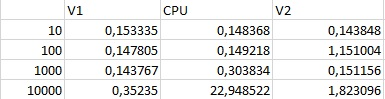
\includegraphics[height=3cm]{waarden.jpg}}
	\end{figure}
	\begin{figure}[htbp]
		\caption{Grafiek}
		\label{tabel}
		\centerline{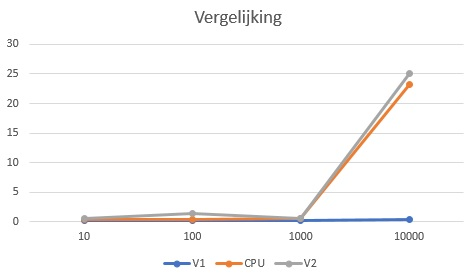
\includegraphics[height=7cm]{grafiek.jpg}}
	\end{figure}

\end{document}